\documentclass[journal]{IEEEtran}

\usepackage[T1]{fontenc}
\usepackage{amsmath,amssymb,amsthm}
\usepackage{booktabs}
\usepackage{array}
\newcolumntype{L}[1]{>{\raggedright\arraybackslash}p{#1}}
\usepackage{cite}
\usepackage{graphicx}
\usepackage{xcolor}
\usepackage[hyphens]{url}
\usepackage[hidelinks]{hyperref}
\usepackage{balance}

\graphicspath{{figures/}}

\newtheorem{lemma}{Lemma}
\newtheorem{proposition}{Proposition}
\theoremstyle{remark}
\newtheorem{remark}{Remark}

\newcommand{\aperp}{\alpha_{\perp}}
\newcommand{\Dtot}{D^{\rm tot}}
\newcommand{\Dfro}{D^{\rm fro}}

% generated by experiments/cdw_hardening/CDWH_NUMBERS.py - do not edit
\newcommand{\altAFrac}{0.00}
\newcommand{\altAGflFracSamePolicies}{0.71}
\newcommand{\altAVerdict}{MODEL-SPECIFIC}
\newcommand{\altAltCases}{488}
\newcommand{\altAltFracInitOkCore}{1.00}
\newcommand{\altAltInitResidualMax}{0.00}
\newcommand{\altBAltMeanFracStableCtxEm}{0.51}
\newcommand{\altBEmFrac}{0.00}
\newcommand{\altBFrac}{0.00}
\newcommand{\altBVerdict}{MODEL-SPECIFIC}
\newcommand{\altCMedianDiff}{0.20}
\newcommand{\altCMedianKendall}{0.06}
\newcommand{\altCMedianRhoAltfd}{0.99}
\newcommand{\altCMedianRhoS}{0.79}
\newcommand{\altCMedianSpearman}{0.13}
\newcommand{\altCNBelow}{3}
\newcommand{\altCVerdict}{TRANSFERS}
\newcommand{\altDFracTopAgree}{0.71}
\newcommand{\altDVerdict}{PARTIAL}
\newcommand{\altENPairs}{29}
\newcommand{\altEPooledSignAgree}{1.00}
\newcommand{\altEVerdict}{TRANSFERS}
\newcommand{\altEmN}{7}
\newcommand{\altEmPol}{N04}
\newcommand{\altEmRev}{1}
\newcommand{\altEmStab}{3}
\newcommand{\altNPoliciesEvaluated}{8}
\newcommand{\altNTestedPolicies}{7}
\newcommand{\bothCDisc}{0.40}
\newcommand{\bothCNew}{0.37}
\newcommand{\bothCOld}{0.28}
\newcommand{\cntADisc}{15/15}
\newcommand{\cntANew}{19/19}
\newcommand{\cntAOld}{18/18}
\newcommand{\cntArbDisc}{15/15}
\newcommand{\cntArbNew}{19/19}
\newcommand{\cntArbOld}{18/18}
\newcommand{\cntBDisc}{14/15}
\newcommand{\cntBNew}{18/19}
\newcommand{\cntBOld}{16/18}
\newcommand{\cntCDisc}{14/15}
\newcommand{\cntCNew}{17/19}
\newcommand{\cntCOld}{16/18}
\newcommand{\cntDDisc}{14/15}
\newcommand{\cntDNew}{17/19}
\newcommand{\cntDOld}{16/18}
\newcommand{\contMatch}{100\%}
\newcommand{\contN}{60}
\newcommand{\corRobust}{none}
\newcommand{\covADisc}{1.00}
\newcommand{\covANew}{1.00}
\newcommand{\covAOld}{1.00}
\newcommand{\covArbDisc}{1.00}
\newcommand{\covArbNew}{1.00}
\newcommand{\covArbOld}{1.00}
\newcommand{\covBDisc}{0.93}
\newcommand{\covBNew}{0.95}
\newcommand{\covBOld}{0.89}
\newcommand{\covCDisc}{0.93}
\newcommand{\covCNew}{0.89}
\newcommand{\covCNewHi}{1.00}
\newcommand{\covCNewLo}{0.74}
\newcommand{\covCOld}{0.89}
\newcommand{\covDDisc}{0.93}
\newcommand{\covDNew}{0.89}
\newcommand{\covDOld}{0.89}
\newcommand{\creDisc}{34}
\newcommand{\creNew}{3}
\newcommand{\creOld}{8}
\newcommand{\dirCboth}{7}
\newcommand{\dirCds}{15}
\newcommand{\dirCsd}{9}
\newcommand{\dirDboth}{3}
\newcommand{\dirDds}{14}
\newcommand{\dirDsd}{6}
\newcommand{\distRho}{0.31}
\newcommand{\dtotDbl}{0.992}
\newcommand{\dtotOut}{0.885}
\newcommand{\dtotOutTop}{0.80}
\newcommand{\dtotTopoNpol}{6}
\newcommand{\emSqNew}{18/19}
\newcommand{\emSqOld}{16/18}
\newcommand{\exDone}{+0.053}
\newcommand{\exDoneAbs}{0.053}
\newcommand{\exDtwo}{0.042}
\newcommand{\exHzOne}{0.64}
\newcommand{\exHzTwo}{0.74}
\newcommand{\exMac}{0.97}
\newcommand{\fastQhi}{3456}
\newcommand{\fastQlo}{20}
\newcommand{\fastQmed}{176}
\newcommand{\fastRealShare}{99\%}
\newcommand{\gapBelowMag}{37\%}
\newcommand{\gapCov}{16/19}
\newcommand{\gbEMTtwosignflipp}{0.000}
\newcommand{\gbEMdifflo}{0.484}
\newcommand{\gbEMfraccondDtotalbeatseverystatic}{1.000}
\newcommand{\gbEMmeandiff}{0.567}
\newcommand{\gbEMmedianconcordDtotal}{0.980}
\newcommand{\gbEMmedianconcordSone}{0.705}
\newcommand{\gbEMmediandiff}{0.488}
\newcommand{\gbEMmediandiffvsoraclestatic}{0.487}
\newcommand{\gbEMmediankendallDtotal}{0.929}
\newcommand{\gbEMmediankendallSone}{0.391}
\newcommand{\gbEMmedianndcgDtotal}{0.994}
\newcommand{\gbEMmedianndcgSone}{0.601}
\newcommand{\gbEMmedianrhoDconv}{0.006}
\newcommand{\gbEMmedianrhoDfrozen}{0.898}
\newcommand{\gbEMmedianrhoDtotal}{0.988}
\newcommand{\gbEMmedianrhoSone}{0.498}
\newcommand{\gbEMmedianrhooraclestatic}{0.499}
\newcommand{\gbEMmediansignaccDtotal}{1.000}
\newcommand{\gbEMmediansignaccSone}{nan}
\newcommand{\gbEMmediantopfiveDtotal}{1.000}
\newcommand{\gbEMmediantopfiveSone}{0.200}
\newcommand{\gbEMmediantopthreeDtotal}{1.000}
\newcommand{\gbEMmediantopthreeSone}{0.000}
\newcommand{\gbEMn}{61}
\newcommand{\gbEMnclusters}{27}
\newcommand{\gbPreregCiHi}{0.608}
\newcommand{\gbPreregCiLo}{0.477}
\newcommand{\gbPrimaryCiHi}{0.638}
\newcommand{\gbPrimaryCiLo}{0.484}
\newcommand{\gbSAMETtwosignflipp}{0.000}
\newcommand{\gbSAMEdifflo}{0.485}
\newcommand{\gbSAMEfraccondDtotalbeatseverystatic}{1.000}
\newcommand{\gbSAMEmeandiff}{0.575}
\newcommand{\gbSAMEmedianconcordDtotal}{0.981}
\newcommand{\gbSAMEmedianconcordSone}{0.705}
\newcommand{\gbSAMEmediandiff}{0.490}
\newcommand{\gbSAMEmediandiffvsoraclestatic}{0.489}
\newcommand{\gbSAMEmediankendallDtotal}{0.929}
\newcommand{\gbSAMEmediankendallSone}{0.389}
\newcommand{\gbSAMEmedianndcgDtotal}{0.994}
\newcommand{\gbSAMEmedianndcgSone}{0.596}
\newcommand{\gbSAMEmedianrhoDconv}{0.004}
\newcommand{\gbSAMEmedianrhoDfrozen}{0.897}
\newcommand{\gbSAMEmedianrhoDtotal}{0.988}
\newcommand{\gbSAMEmedianrhoSone}{0.495}
\newcommand{\gbSAMEmedianrhooraclestatic}{0.496}
\newcommand{\gbSAMEmediansignaccDtotal}{1.000}
\newcommand{\gbSAMEmediansignaccSone}{nan}
\newcommand{\gbSAMEmediantopfiveDtotal}{1.000}
\newcommand{\gbSAMEmediantopfiveSone}{0.200}
\newcommand{\gbSAMEmediantopthreeDtotal}{1.000}
\newcommand{\gbSAMEmediantopthreeSone}{0.000}
\newcommand{\gbSAMEn}{64}
\newcommand{\gbSAMEnclusters}{28}
\newcommand{\gbVnineTtwosignflipp}{0.000}
\newcommand{\gbVninedifflo}{1.132}
\newcommand{\gbVninefraccondDtotalbeatseverystatic}{1.000}
\newcommand{\gbVninemeandiff}{1.183}
\newcommand{\gbVninemedianconcordDtotal}{0.978}
\newcommand{\gbVninemedianconcordSone}{0.433}
\newcommand{\gbVninemediandiff}{1.180}
\newcommand{\gbVninemediandiffvsoraclestatic}{0.672}
\newcommand{\gbVninemediankendallDtotal}{0.953}
\newcommand{\gbVninemediankendallSone}{-0.133}
\newcommand{\gbVninemedianndcgDtotal}{1.000}
\newcommand{\gbVninemedianndcgSone}{0.809}
\newcommand{\gbVninemedianrhoDconv}{-0.195}
\newcommand{\gbVninemedianrhoDfrozen}{0.943}
\newcommand{\gbVninemedianrhoDtotal}{0.994}
\newcommand{\gbVninemedianrhoSone}{-0.183}
\newcommand{\gbVninemedianrhooraclestatic}{0.326}
\newcommand{\gbVninemediansignaccDtotal}{0.977}
\newcommand{\gbVninemediansignaccSone}{nan}
\newcommand{\gbVninemediantopfiveDtotal}{1.000}
\newcommand{\gbVninemediantopfiveSone}{0.000}
\newcommand{\gbVninemediantopthreeDtotal}{1.000}
\newcommand{\gbVninemediantopthreeSone}{0.000}
\newcommand{\gbVninen}{24}
\newcommand{\gbVninenclusters}{24}
\newcommand{\gbfreshdrawsTtwosignflipp}{0.121}
\newcommand{\gbfreshdrawsdifflo}{0.483}
\newcommand{\gbfreshdrawsfraccondDtotalbeatseverystatic}{1.000}
\newcommand{\gbfreshdrawsmeandiff}{0.510}
\newcommand{\gbfreshdrawsmedianconcordDtotal}{0.978}
\newcommand{\gbfreshdrawsmedianconcordSone}{0.706}
\newcommand{\gbfreshdrawsmediandiff}{0.484}
\newcommand{\gbfreshdrawsmediandiffvsoraclestatic}{0.484}
\newcommand{\gbfreshdrawsmediankendallDtotal}{0.925}
\newcommand{\gbfreshdrawsmediankendallSone}{0.395}
\newcommand{\gbfreshdrawsmedianndcgDtotal}{0.991}
\newcommand{\gbfreshdrawsmedianndcgSone}{0.577}
\newcommand{\gbfreshdrawsmedianrhoDconv}{-0.071}
\newcommand{\gbfreshdrawsmedianrhoDfrozen}{0.901}
\newcommand{\gbfreshdrawsmedianrhoDtotal}{0.986}
\newcommand{\gbfreshdrawsmedianrhoSone}{0.503}
\newcommand{\gbfreshdrawsmedianrhooraclestatic}{0.504}
\newcommand{\gbfreshdrawsmediansignaccDtotal}{1.000}
\newcommand{\gbfreshdrawsmediansignaccSone}{nan}
\newcommand{\gbfreshdrawsmediantopfiveDtotal}{0.800}
\newcommand{\gbfreshdrawsmediantopfiveSone}{0.200}
\newcommand{\gbfreshdrawsmediantopthreeDtotal}{0.667}
\newcommand{\gbfreshdrawsmediantopthreeSone}{0.000}
\newcommand{\gbfreshdrawsn}{40}
\newcommand{\gbfreshdrawsnclusters}{4.000}
\newcommand{\gbgOneTenTtwosignflipp}{0.000}
\newcommand{\gbgOneTendifflo}{0.498}
\newcommand{\gbgOneTenfraccondDtotalbeatseverystatic}{1.000}
\newcommand{\gbgOneTenmeandiff}{0.594}
\newcommand{\gbgOneTenmedianconcordDtotal}{1.000}
\newcommand{\gbgOneTenmedianconcordSone}{0.724}
\newcommand{\gbgOneTenmediandiff}{0.503}
\newcommand{\gbgOneTenmediandiffvsoraclestatic}{0.502}
\newcommand{\gbgOneTenmediankendallDtotal}{0.985}
\newcommand{\gbgOneTenmediankendallSone}{0.387}
\newcommand{\gbgOneTenmedianndcgDtotal}{1.000}
\newcommand{\gbgOneTenmedianndcgSone}{0.642}
\newcommand{\gbgOneTenmedianrhoDconv}{0.060}
\newcommand{\gbgOneTenmedianrhoDfrozen}{0.891}
\newcommand{\gbgOneTenmedianrhoDtotal}{0.999}
\newcommand{\gbgOneTenmedianrhoSone}{0.495}
\newcommand{\gbgOneTenmedianrhooraclestatic}{0.496}
\newcommand{\gbgOneTenmediansignaccDtotal}{1.000}
\newcommand{\gbgOneTenmediansignaccSone}{nan}
\newcommand{\gbgOneTenmediantopfiveDtotal}{1.000}
\newcommand{\gbgOneTenmediantopfiveSone}{0.200}
\newcommand{\gbgOneTenmediantopthreeDtotal}{1.000}
\newcommand{\gbgOneTenmediantopthreeSone}{0.333}
\newcommand{\gbgOneTenn}{64}
\newcommand{\gbgOneTennclusters}{28}
\newcommand{\gbgOneTwentyFiveTtwosignflipp}{0.000}
\newcommand{\gbgOneTwentyFivedifflo}{0.489}
\newcommand{\gbgOneTwentyFivefraccondDtotalbeatseverystatic}{1.000}
\newcommand{\gbgOneTwentyFivemeandiff}{0.592}
\newcommand{\gbgOneTwentyFivemedianconcordDtotal}{0.998}
\newcommand{\gbgOneTwentyFivemedianconcordSone}{0.713}
\newcommand{\gbgOneTwentyFivemediandiff}{0.500}
\newcommand{\gbgOneTwentyFivemediandiffvsoraclestatic}{0.496}
\newcommand{\gbgOneTwentyFivemediankendallDtotal}{0.961}
\newcommand{\gbgOneTwentyFivemediankendallSone}{0.390}
\newcommand{\gbgOneTwentyFivemedianndcgDtotal}{1.000}
\newcommand{\gbgOneTwentyFivemedianndcgSone}{0.629}
\newcommand{\gbgOneTwentyFivemedianrhoDconv}{0.056}
\newcommand{\gbgOneTwentyFivemedianrhoDfrozen}{0.894}
\newcommand{\gbgOneTwentyFivemedianrhoDtotal}{0.995}
\newcommand{\gbgOneTwentyFivemedianrhoSone}{0.495}
\newcommand{\gbgOneTwentyFivemedianrhooraclestatic}{0.497}
\newcommand{\gbgOneTwentyFivemediansignaccDtotal}{1.000}
\newcommand{\gbgOneTwentyFivemediansignaccSone}{nan}
\newcommand{\gbgOneTwentyFivemediantopfiveDtotal}{1.000}
\newcommand{\gbgOneTwentyFivemediantopfiveSone}{0.200}
\newcommand{\gbgOneTwentyFivemediantopthreeDtotal}{1.000}
\newcommand{\gbgOneTwentyFivemediantopthreeSone}{0.000}
\newcommand{\gbgOneTwentyFiven}{64}
\newcommand{\gbgOneTwentyFivenclusters}{28}
\newcommand{\gbnewpoliciesTtwosignflipp}{0.000}
\newcommand{\gbnewpoliciesdifflo}{0.588}
\newcommand{\gbnewpoliciesfraccondDtotalbeatseverystatic}{1.000}
\newcommand{\gbnewpoliciesmeandiff}{0.708}
\newcommand{\gbnewpoliciesmedianconcordDtotal}{0.999}
\newcommand{\gbnewpoliciesmedianconcordSone}{0.616}
\newcommand{\gbnewpoliciesmediandiff}{0.741}
\newcommand{\gbnewpoliciesmediandiffvsoraclestatic}{0.546}
\newcommand{\gbnewpoliciesmediankendallDtotal}{0.962}
\newcommand{\gbnewpoliciesmediankendallSone}{0.182}
\newcommand{\gbnewpoliciesmedianndcgDtotal}{0.999}
\newcommand{\gbnewpoliciesmedianndcgSone}{0.636}
\newcommand{\gbnewpoliciesmedianrhoDconv}{0.304}
\newcommand{\gbnewpoliciesmedianrhoDfrozen}{0.712}
\newcommand{\gbnewpoliciesmedianrhoDtotal}{0.996}
\newcommand{\gbnewpoliciesmedianrhoSone}{0.256}
\newcommand{\gbnewpoliciesmedianrhooraclestatic}{0.445}
\newcommand{\gbnewpoliciesmediansignaccDtotal}{1.000}
\newcommand{\gbnewpoliciesmediansignaccSone}{nan}
\newcommand{\gbnewpoliciesmediantopfiveDtotal}{1.000}
\newcommand{\gbnewpoliciesmediantopfiveSone}{0.200}
\newcommand{\gbnewpoliciesmediantopthreeDtotal}{1.000}
\newcommand{\gbnewpoliciesmediantopthreeSone}{0.333}
\newcommand{\gbnewpoliciesn}{24}
\newcommand{\gbnewpoliciesnclusters}{24}
\newcommand{\gbnoneartieTtwosignflipp}{0.000}
\newcommand{\gbnoneartiedifflo}{0.484}
\newcommand{\gbnoneartiefraccondDtotalbeatseverystatic}{1.000}
\newcommand{\gbnoneartiemeandiff}{0.572}
\newcommand{\gbnoneartiemedianconcordDtotal}{0.981}
\newcommand{\gbnoneartiemedianconcordSone}{0.705}
\newcommand{\gbnoneartiemediandiff}{0.488}
\newcommand{\gbnoneartiemediandiffvsoraclestatic}{0.487}
\newcommand{\gbnoneartiemediankendallDtotal}{0.929}
\newcommand{\gbnoneartiemediankendallSone}{0.390}
\newcommand{\gbnoneartiemedianndcgDtotal}{0.994}
\newcommand{\gbnoneartiemedianndcgSone}{0.602}
\newcommand{\gbnoneartiemedianrhoDconv}{0.016}
\newcommand{\gbnoneartiemedianrhoDfrozen}{0.897}
\newcommand{\gbnoneartiemedianrhoDtotal}{0.988}
\newcommand{\gbnoneartiemedianrhoSone}{0.498}
\newcommand{\gbnoneartiemedianrhooraclestatic}{0.499}
\newcommand{\gbnoneartiemediansignaccDtotal}{1.000}
\newcommand{\gbnoneartiemediansignaccSone}{nan}
\newcommand{\gbnoneartiemediantopfiveDtotal}{1.000}
\newcommand{\gbnoneartiemediantopfiveSone}{0.200}
\newcommand{\gbnoneartiemediantopthreeDtotal}{1.000}
\newcommand{\gbnoneartiemediantopthreeSone}{0.000}
\newcommand{\gbnoneartien}{62}
\newcommand{\gbnoneartienclusters}{28}
\newcommand{\gbpreregTtwosignflipp}{0.061}
\newcommand{\gbpreregdifflo}{0.477}
\newcommand{\gbpreregfraccondDtotalbeatseverystatic}{1.000}
\newcommand{\gbpreregmeandiff}{0.551}
\newcommand{\gbpreregmedianconcordDtotal}{0.980}
\newcommand{\gbpreregmedianconcordSone}{0.704}
\newcommand{\gbpreregmediandiff}{0.492}
\newcommand{\gbpreregmediandiffvsoraclestatic}{0.492}
\newcommand{\gbpreregmediankendallDtotal}{0.924}
\newcommand{\gbpreregmediankendallSone}{0.386}
\newcommand{\gbpreregmedianndcgDtotal}{0.986}
\newcommand{\gbpreregmedianndcgSone}{0.629}
\newcommand{\gbpreregmedianrhoDconv}{-0.046}
\newcommand{\gbpreregmedianrhoDfrozen}{0.913}
\newcommand{\gbpreregmedianrhoDtotal}{0.985}
\newcommand{\gbpreregmedianrhoSone}{0.491}
\newcommand{\gbpreregmedianrhooraclestatic}{0.491}
\newcommand{\gbpreregmediansignaccDtotal}{1.000}
\newcommand{\gbpreregmediansignaccSone}{nan}
\newcommand{\gbpreregmediantopfiveDtotal}{1.000}
\newcommand{\gbpreregmediantopfiveSone}{0.200}
\newcommand{\gbpreregmediantopthreeDtotal}{0.833}
\newcommand{\gbpreregmediantopthreeSone}{0.000}
\newcommand{\gbpreregn}{8.000}
\newcommand{\gbpreregnclusters}{6.000}
\newcommand{\gbprimaryTtwosignflipp}{0.000}
\newcommand{\gbprimarydifflo}{0.484}
\newcommand{\gbprimaryfraccondDtotalbeatseverystatic}{1.000}
\newcommand{\gbprimarymeandiff}{0.585}
\newcommand{\gbprimarymedianconcordDtotal}{0.980}
\newcommand{\gbprimarymedianconcordSone}{0.705}
\newcommand{\gbprimarymediandiff}{0.489}
\newcommand{\gbprimarymediandiffvsoraclestatic}{0.487}
\newcommand{\gbprimarymediankendallDtotal}{0.929}
\newcommand{\gbprimarymediankendallSone}{0.389}
\newcommand{\gbprimarymedianndcgDtotal}{0.994}
\newcommand{\gbprimarymedianndcgSone}{0.607}
\newcommand{\gbprimarymedianrhoDconv}{0.034}
\newcommand{\gbprimarymedianrhoDfrozen}{0.895}
\newcommand{\gbprimarymedianrhoDtotal}{0.987}
\newcommand{\gbprimarymedianrhoSone}{0.497}
\newcommand{\gbprimarymedianrhooraclestatic}{0.499}
\newcommand{\gbprimarymediansignaccDtotal}{1.000}
\newcommand{\gbprimarymediansignaccSone}{nan}
\newcommand{\gbprimarymediantopfiveDtotal}{1.000}
\newcommand{\gbprimarymediantopfiveSone}{0.200}
\newcommand{\gbprimarymediantopthreeDtotal}{1.000}
\newcommand{\gbprimarymediantopthreeSone}{0.000}
\newcommand{\gbprimaryn}{64}
\newcommand{\gbprimarynclusters}{28}
\newcommand{\gscrSeqEM}{0.68}
\newcommand{\gscrSeqFull}{0.76}
\newcommand{\heightFlipCond}{100\%}
\newcommand{\heightKendall}{0.75}
\newcommand{\heightMaterial}{28\%}
\newcommand{\ivLinks}{100\%}
\newcommand{\ivN}{4048}
\newcommand{\lSevenEC}{1.00}
\newcommand{\lSevenEMC}{1.00}
\newcommand{\lSevenEMEC}{0.00}
\newcommand{\lSevenEMEMC}{0.70}
\newcommand{\lSevenEMEMf}{0.50}
\newcommand{\lSevenEMEMu}{0.60}
\newcommand{\lSevenEMf}{0.90}
\newcommand{\lSevenEMu}{0.80}
\newcommand{\layersPos}{7}
\newcommand{\locoAll}{0.943}
\newcommand{\locoDraws}{0.959}
\newcommand{\locoMarginDraws}{0.03}
\newcommand{\locoMarginNew}{0.17}
\newcommand{\locoNew}{0.818}
\newcommand{\locoTopfive}{0.80}
\newcommand{\minRegEM}{0.03}
\newcommand{\minRegFull}{0.34}
\newcommand{\mixCov}{-30\%}
\newcommand{\mixNewN}{19}
\newcommand{\mixNewP}{0.016}
\newcommand{\mixNewRho}{0.55}
\newcommand{\mixOldFixedRho}{0.21}
\newcommand{\mixOldOrigRho}{0.66}
\newcommand{\mixShareC}{33\%}
\newcommand{\mixVarC}{19\%}
\newcommand{\mixVarCtrl}{24\%}
\newcommand{\mixVarFreq}{106\%}
\newcommand{\nDiscStable}{15}
\newcommand{\nDiscUnstable}{0}
\newcommand{\nElig}{8}
\newcommand{\nEligClusters}{6}
\newcommand{\nNewStable}{19}
\newcommand{\nNewUnstable}{5}
\newcommand{\nOldStable}{18}
\newcommand{\nOldUnstable}{6}
\newcommand{\nOrders}{24}
\newcommand{\newCds}{2172}
\newcommand{\newCemClean}{94\%}
\newcommand{\newCmagMed}{0.013}
\newcommand{\newCmagQone}{0.011}
\newcommand{\newCmagQthree}{0.017}
\newcommand{\newCpairs}{3263}
\newcommand{\newCsd}{1091}
\newcommand{\noStable}{22\%}
\newcommand{\nodeLoadDom}{61\%}
\newcommand{\nodeLoadRatio}{1.30}
\newcommand{\nodeRone}{2.2e-07}
\newcommand{\nodeVsetDom}{100\%}
\newcommand{\orderKendall}{0.72}
\newcommand{\partIq}{0.36}
\newcommand{\partTheta}{0.39}
\newcommand{\pstarEMDisc}{0.98}
\newcommand{\pstarEMNew}{0.97}
\newcommand{\pstarEMOld}{0.97}
\newcommand{\pstarFULLDisc}{0.79}
\newcommand{\pstarFULLNew}{0.75}
\newcommand{\pstarFULLOld}{0.75}
\newcommand{\pstarNewHi}{0.78}
\newcommand{\pstarNewLo}{0.74}
\newcommand{\pstarSAMEDisc}{0.98}
\newcommand{\pstarSAMENew}{0.98}
\newcommand{\pstarSAMEOld}{0.98}
\newcommand{\rZeroMax}{$2.1\times10^{-7}$}
\newcommand{\regPlainFeas}{0.27}
\newcommand{\regScreened}{0.065}
\newcommand{\regretEMDisc}{0.03}
\newcommand{\regretEMNew}{0.03}
\newcommand{\regretEMOld}{0.03}
\newcommand{\regretFULLDisc}{0.36}
\newcommand{\regretFULLNew}{0.38}
\newcommand{\regretFULLOld}{0.37}
\newcommand{\regretFastShare}{92\%}
\newcommand{\regretNbad}{2265}
\newcommand{\regretNewHi}{0.39}
\newcommand{\regretNewLo}{0.36}
\newcommand{\regretNfast}{2089}
\newcommand{\regretSAMEDisc}{0.02}
\newcommand{\regretSAMENew}{0.02}
\newcommand{\regretSAMEOld}{0.02}
\newcommand{\revCdistinct}{87}
\newcommand{\revCds}{1990}
\newcommand{\revCemClean}{96\%}
\newcommand{\revCmax}{0.042}
\newcommand{\revCpairs}{3067}
\newcommand{\revCsd}{1077}
\newcommand{\revDboth}{3}
\newcommand{\revDds}{1800}
\newcommand{\revDmed}{0.013}
\newcommand{\revDpairs}{2543}
\newcommand{\revDsd}{743}
\newcommand{\revZetaMed}{0.32}
\newcommand{\revZetaQone}{0.27}
\newcommand{\revZetaQthree}{0.39}
\newcommand{\shiftPstar}{-0.002}
\newcommand{\shiftPstarHi}{0.041}
\newcommand{\shiftPstarLo}{-0.036}
\newcommand{\shiftRegret}{0.007}
\newcommand{\shiftRegretHi}{0.029}
\newcommand{\shiftRegretLo}{-0.020}
\newcommand{\statFiedlerFrac}{0.25}
\newcommand{\statFiedlerRho}{-0.50}
\newcommand{\statGscrHFrac}{0.31}
\newcommand{\statGscrHRho}{-0.54}
\newcommand{\statKirchhoffFrac}{0.38}
\newcommand{\statKirchhoffRho}{0.56}
\newcommand{\statLossesFrac}{0.38}
\newcommand{\statLossesRho}{0.55}
\newcommand{\statMaxFlowFrac}{0.00}
\newcommand{\statMaxFlowRho}{0.39}
\newcommand{\statMeanReffCoreFrac}{0.06}
\newcommand{\statMeanReffCoreRho}{0.41}
\newcommand{\statMinScrCoreFrac}{0.25}
\newcommand{\statMinScrCoreRho}{-0.54}
\newcommand{\sweepJumpHi}{109804}
\newcommand{\sweepJumpLo}{3773}
\newcommand{\sweepN}{6}
\newcommand{\sweepSigHi}{0.007}
\newcommand{\sweepSigLo}{0.002}
\newcommand{\tOneK}{19}
\newcommand{\tOneN}{19}
\newcommand{\tOneP}{1.9e-06}
\newcommand{\tOnePholm}{5.7e-06}
\newcommand{\tThreeP}{0.016}
\newcommand{\tThreePholm}{0.033}
\newcommand{\tTwoP}{0.061}
\newcommand{\tTwoPholm}{0.061}
\newcommand{\tauCthree}{10}
\newcommand{\tauCtwo}{15}
\newcommand{\tauDthree}{5}
\newcommand{\tauDtwo}{11}
\newcommand{\timeDer}{1.46}
\newcommand{\timeFin}{0.61}
\newcommand{\topoFastHfour}{50}
\newcommand{\topoNcreate}{45}
\newcommand{\topoNfastCreate}{0}
\newcommand{\topoNpol}{16}
\newcommand{\topoRemovalPfour}{dbl13, dbl43, dbl1, dbl0}
\newcommand{\transDiagAcc}{0.76}
\newcommand{\transDiagReg}{0.38}
\newcommand{\transN}{52}
\newcommand{\transOffAcc}{0.73}
\newcommand{\transOffReg}{0.40}
\newcommand{\withinDblFiedler}{0.00}
\newcommand{\withinOutLosses}{0.44}


\title{Portfolio-Conditioned Dynamic Weakness and\\ Reinforcement Ranking in
Inverter-Rich Power Networks}

\author{Jorge L.~Mayorga Taborda%
\thanks{J. L. Mayorga Taborda is with the Department of Electrical and
Electronic Engineering, Universidad de los Andes, Bogot\'a, Colombia
(e-mail: jl.mayorga@uniandes.edu.co).}%
}

\begin{document}
\maketitle

\begin{abstract}
When synchronous generators (SGs) are replaced by grid-following converters
(GFLs) unit by unit, a planner needs the small-signal effect of the next
replacement and of the next reinforcement in the portfolio at hand. We study
these marginal effects on the IEEE 39-bus system with a documented GFL model:
all $2^9$ replacement portfolios at 63 controller policies, 24 of them a
preregistered maximin holdout. In \cntDNew{} base-stable holdout policies the
same replacement moves the same tracked electromechanical mode in opposite
directions in two nested stable portfolios. The effects are small (median
\revDmed~s$^{-1}$, about 0.3\,\% damping ratio) and vanish above
0.05~s$^{-1}$; by the classical chain identity each reversal locates an
interaction term of the matching sign. A fixed ranking of units makes a
materially worse next choice in \regretFULLNew{} of decisions, but nearly all of
these errors are replacements that cross a singularity-type aperiodic
instability of the phasor model at high converter share; screened for stability,
a fixed ranking errs in \regScreened. For branch reinforcement, the
re-equilibrated eigenvalue sensitivity of the current portfolio ranks finite
reinforcements with median Spearman \gbnewpoliciesmedianrhoDtotal{} across the
new policies, against \gbnewpoliciesmedianrhoDfrozen{} for the frozen-operating-point
derivative, \locoNew{} for a fixed list learned from other conditions and at
most \gbnewpoliciesmedianrhooraclestatic{} for static strength indices; it also
ranks branch doublings and outages. With a frozen WECC library GFL the ranking
method carries over, while the reversals and the branch ranking do not.
\end{abstract}

\begin{IEEEkeywords}
Grid-following converters, small-signal stability, eigenvalue sensitivity,
grid strength, replacement planning, set functions.
\end{IEEEkeywords}

% =========================================================================
\section{Introduction}

\IEEEPARstart{G}{rid-strength} indices summarize how well a network supports
converter-interfaced resources. Single-infeed short-circuit ratios yield
context-free lists of weak buses; multi-infeed generalizations---the
site-dependent SCR~\cite{wu2018sdscr}, the generalized
SCR~\cite{xin2016gscr,dong2019gscr,zhou2023heterogeneous}, the generalized
operational SCR~\cite{liu2024goscr}, small-signal strength of all-inverter
systems~\cite{ma2024strength} and impedance
metrics~\cite{henderson2024gsim,lamrani2025fagim}---are defined for a given set
of converter buses and are thus portfolio-conditioned static screens. Modal
participation~\cite{ebrahimzadeh2018busPF,zhu2022greybox} and impedance-based
eigenvalue sensitivities~\cite{zhu2023rootcause} rank dynamic criticality.

Retirement poses a sequential question. Units are replaced one at a time, and
the planner must decide which unit to replace next \emph{given} those already
replaced, and which branch to reinforce \emph{given} the resulting portfolio. The
object is the contextual marginal
\begin{equation}\label{eq:marg}
\Delta_i\aperp(S)=\aperp(S\cup\{i\})-\aperp(S),
\end{equation}
the change of the rightmost transverse eigenvalue's real part when unit $i$ is
replaced in portfolio $S$. It has long been known that displacing SGs by
converters improves some electromechanical modes and degrades
others~\cite{gautam2009dfig}, that rising converter penetration changes the
participation in inter-area modes and adds converter-dominated
modes~\cite{quintero2014converter}, that the small-signal effect of converters
depends on the mix and dispatch in which they
operate~\cite{li2023intrinsic,markovic2021lowinertia,stanojev2023vim,desai2026dispatch},
and that a branch reinforcement can reduce linear stability
(Braess-type behavior~\cite{coletta2016braess,schafer2022braess};
operating-point-dependent edge weights~\cite{song2018network}). Eigenvalue
sensitivities with a re-solved operating point are
classical~\cite{smed1993feasible,nam2000eigsens,mendozaarmenta2016redispatch,li2019opsens},
and a recent preprint chains them to line admittances~\cite{joswigjones2026sens};
topology switching changes small-signal margins~\cite{saric2015rapid,li2018switching};
and natural dynamic set functions are known to violate
sub- or supermodularity~\cite{summers2016submodularity,olshevsky2018nonsupermodularity,summers2019greedy}.

This paper is an empirical, preregistered study on one benchmark. It
contributes four findings, each stated with its limits:
\begin{itemize}
\item[C1)] \emph{Nested same-mode reversal.} The same replacement moves the same
tracked electromechanical (EM) mode in opposite directions in two nested stable
portfolios in \cntDNew{} base-stable policies of a new holdout. The effects are
about one hundredth of s$^{-1}$ and disappear above 0.05~s$^{-1}$.
\item[C2)] \emph{Why fixed unit rankings fail here.} An oracle fixed ranking
errs materially in about a third of next-replacement decisions, but the errors
are almost all replacements that cross an aperiodic, singularity-type instability
of the phasor model at high converter share; with a stability screen a fixed
ranking is nearly adequate, and a portfolio-conditioned gSCR screen is not.
\item[C3)] \emph{Portfolio-conditioned reinforcement ranking.} The re-equilibrated
sensitivity of the current portfolio ranks finite reinforcements, doublings and
outages better than the frozen derivative, a fixed list learned from other
conditions, and static indices; the operating-point term vanishes for controller
coordinates and matters for network coordinates.
\item[C4)] \emph{Boundaries.} Single branch actions remove and create EM
incompatibilities; with a frozen WECC library GFL the ranking method carries over
but the reversals and the ranking do not.
\end{itemize}
The study is phasor-domain small-signal analysis; no electromagnetic-transient
claim is made.

% =========================================================================
\section{Problem Formulation}\label{sec:model}

\subsection{Model}
The network is the IEEE 39-bus system~\cite{athay1979} (46 branches, ten SGs,
bus 39 an interconnection equivalent) in phasor form with constant-power loads.
The system is the index-one DAE $\dot x=f(x,z;p)$, $0=g(x,z;p)$ with device
states $x$, rectangular bus voltages $z$ and parameters $p$; at an equilibrium
the reduced Jacobian is $A=f_x-f_zg_z^{-1}g_x$. Each SG is a two-axis
machine~\cite{sauer1998} with $D=0$, constant mechanical power, a first-order AVR
$T_E\dot e_{fd}=K_A(v_{\rm ref}+v_s-|V|)-e_{fd}$ and a power-input stabilizer.
Machine, AVR and PSS data, ratings and the power flow are taken from the IEEE
39-bus dynamic case distributed with ANDES~\cite{cui2021andes} (GENROU records
used in two-axis form, IEEEX1 gain $K_A$ and time constant $T_E$, IEEEST
stabilizer); Table~\ref{tab:param} lists the controller values. Each
GFL has a synchronous-reference-frame PLL, filtered power measurements, PI outer
and inner loops behind a filter reactance, and a leaky Q/V regulator
$q_{\rm cmd}=k_{p,v}\,g\,e+x_v$, $\dot x_v=k_{i,v}\,g\,e-w(x_v-q_{\rm ref})$,
$e=v_{\rm ref}-|V|$, $w=0.05$~rad/s. Converter current limits, DC links and
delays are not modeled.

\begin{table}[!t]
\centering
\caption{Device and benchmark data (per unit on device rating)}\label{tab:param}
\footnotesize
\setlength{\tabcolsep}{3pt}
\begin{tabular}{@{}lL{0.70\columnwidth}@{}}
\toprule
SG & two-axis, $D=0$, constant $P_m$, $M$ 4.9--8.4~s (bus 39: 100~s); AVR $K_A\in\{10.1,40\}$, $T_E$ 0.25--0.95~s by unit; PSS $K_S=-2$, $T_5=1$, $T_6=4.2$, $T_4=0.75$~s\\
PLL & $k_{p,\rm pll}=53$, $k_{i,\rm pll}=1400$\\
GFL loops & $\tau=0.03$~s; outer $0.2/8$; inner $0.25/6$; $x_f=0.15$, $r_f=0.01$\\
Q/V & $k_{p,v}/k_{i,v}=2/20$, leak $w=0.05$~rad/s, gain $g\in[0,1]$\\
Candidates & $V_9=\{30,\dots,38\}$ ($2^9$ portfolios); core $V_4=\{30,33,35,37\}$\\
\bottomrule
\end{tabular}
\end{table}

A \emph{policy} $\theta=(g,k,t,h)$ sets the Q/V gain $g$ of every GFL, a common
scale $k$ of the surviving SGs' AVR gains, a scale $t$ of their AVR time
constants, and a heterogeneity exponent $h$ with $T_{E,i}\mapsto G(T_{E,i}/G)^h$,
$G$ the geometric mean. Replacing unit $i$ installs a GFL with the SG's active
and reactive dispatch and rating (matched dispatch), so the base power flow is
the same for every portfolio. The flagship policy P4 $=(0.03625,1.425,1.5,1)$
makes $V_4$ unstable with a 0.62~Hz critical mode while all its subsets are
stable.

\subsection{Transverse stability}
With $D=0$ and no governors the model has an exact rotation symmetry and a
neutral frequency mode (two structural zero eigenvalues). Stability is evaluated
on the transverse quotient that removes them; $\aperp$ is the largest real part
of the transverse spectrum. A portfolio is STABLE if all transverse eigenvalues
satisfy ${\rm Re}\,\lambda\le-2\times10^{-3}$, UNSTABLE if one has
${\rm Re}\,\lambda\ge2\times10^{-3}$, and unresolved otherwise.

\subsection{Contextual marginals and modal levels}
For a policy $\theta$, $f(S)=\aperp(S;\theta)$ on $S\subseteq V_9$. A marginal
\eqref{eq:marg} is \emph{material} if $|\Delta_if(S)|\ge\tau_{\rm mat}=0.01$~s$^{-1}$
(about 0.2\,\% damping ratio at 0.7~Hz); its sign class is $-1$ (stabilizing),
$0$ or $+1$. Because a change of $\aperp$ can be a jump between modes, each
marginal $(S,i)$ is graded: (A) $S$ is STABLE; (B) the critical mode of $S$ has a
match in $S\cup\{i\}$ that is the critical mode of $S\cup\{i\}$; (C) B, with both
critical frequencies in 0.1--2.0~Hz; (D) for a pair of contexts, C at both, and
their critical modes match each other. Matching uses the modal assurance
criterion (MAC $\ge0.8$) on the 78 rectangular bus-voltage components of the mode
shape (unit norm, phase fixed at the largest entry), among eigenvalues in
0.1--2.0~Hz with ${\rm Re}\ge-1$~s$^{-1}$ plus the critical one, with
$|\Delta f|\le0.15$~Hz. Level D is the ``same mode'' statement.

% =========================================================================
\section{Marginals and Second Differences}\label{sec:theory}

For $S\subseteq V$ and distinct $i,j\notin S$ let
$d_{ij}(S)=f(S\cup\{i,j\})-f(S\cup\{i\})-f(S\cup\{j\})+f(S)=\Delta_if(S\cup\{j\})-\Delta_if(S)$,
the one-step second difference (interaction term). $f$ is submodular if
$\Delta_if(S)\ge\Delta_if(T)$ for $S\subseteq T$, $i\notin T$, equivalently
$d_{ij}(S)\le0$ everywhere, and supermodular with the inequalities
reversed~\cite{topkis1978,lovasz1983,fujishige2005,bach2013}. The following
algebra is classical; we use it to locate interactions, not as a new result.

\begin{lemma}[chain identity]\label{lem:chain}
Let $S_0\subseteq V$, $j_1,\dots,j_m\in V\setminus S_0$ distinct,
$S_r=S_{r-1}\cup\{j_r\}$, and $i\notin S_m$. Then
$\Delta_if(S_m)=\Delta_if(S_0)+\sum_{r=1}^m d_{ij_r}(S_{r-1})$.
\end{lemma}
\begin{IEEEproof}
$d_{ij_r}(S_{r-1})=\Delta_if(S_r)-\Delta_if(S_{r-1})$; sum over $r$.
\end{IEEEproof}

A \emph{nested reversal} of $i$ is a pair $S_1\subsetneq S_2$, $i\notin S_2$,
with $\Delta_if(S_1)$, $\Delta_if(S_2)$ in opposite sign classes; its direction is
s$\to$d (stabilizing at $S_1$, destabilizing at $S_2$) or d$\to$s.

\begin{proposition}\label{prop:abc}
A nested s$\to$d reversal is incompatible with submodularity and a nested d$\to$s
reversal with supermodularity; along the chain from $S_1$ to $S_2$ some term
satisfies $d_{ij_r}\ge D/m$ if $D=\Delta_if(S_2)-\Delta_if(S_1)>0$ ($\le D/m$ if
$D<0$), $m=|S_2\setminus S_1|$.
\end{proposition}
\begin{IEEEproof}
Under submodularity all terms of Lemma~\ref{lem:chain} are nonpositive, so the
marginal cannot increase along a growing chain; supermodularity is symmetric. The
$m$ terms sum to $D$, so the largest is at least $D/m$.
\end{IEEEproof}

The bound holds for every nested pair by construction; its use is to point at an
interaction $d_{ij_r}$ between $i$ and a unit $j_r$ added on the way from $S_1$ to
$S_2$. A reversal between \emph{incomparable} contexts does not contradict
submodularity: on $V=\{i,a,b\}$ with $f(\emptyset)=f(a)=f(b)=f(ab)=0$, $f(i)=2$,
$f(ai)=-1$, $f(bi)=1$, $f(abi)=-2$, all six second differences are nonpositive,
yet $\Delta_if(\{a\})<0<\Delta_if(\{b\})$. That submodular example also contains the
nested d$\to$s reversal $\emptyset\subset\{a\}$, as Proposition~\ref{prop:abc}
allows.

\begin{proposition}[preference drift]\label{prop:drift}
For a chain as in Lemma~\ref{lem:chain} and $i,j\notin S_m$,
$\big(\Delta_if-\Delta_jf\big)(S_m)-\big(\Delta_if-\Delta_jf\big)(S_0)=
\sum_{r=1}^m\big(d_{ik_r}-d_{jk_r}\big)(S_{r-1})$, with $k_r$ the added units.
If the preference between $i$ and $j$ reverses materially, every fixed ranking
errs in one of the two contexts, and some $d_{ik_r}-d_{jk_r}\ge2\tau/m$.
\end{proposition}
\begin{IEEEproof}
Apply Lemma~\ref{lem:chain} to $i$ and $j$ and subtract.
\end{IEEEproof}

\begin{remark}\label{rem:heter}
If $f(S)=h(|S|)+\sum_{k\in S}w_k$ then $d_{ik}=d_{jk}$ and the ranking by $w$ is
exact in every context, whether $h$ is concave or convex. Heterogeneity of
interactions across units is thus necessary for a fixed ranking to fail; the sign
of the interactions is not what matters. Sub- and supermodularity refer to $f$ on
all of $2^V$; the stable portfolios do not form a lattice, so no greedy guarantee
is at stake.
\end{remark}

% =========================================================================
\section{Dynamic Intervention Sensitivity}\label{sec:sens}

Let $w=(x,z,r)$ collect states, bus voltages and freed references $r$. Under
\emph{scheduled-power-and-voltage} (SPR) semantics the references of every unit
are re-solved so that it keeps its scheduled active power and terminal voltage;
the slack machine at bus 39 absorbs the loss change and fixes the angle
reference, and the frequency is the nominal one, which pins the symmetry
directions. The equilibrium solves $R(w;a)=0$. For a simple critical eigenvalue
$\lambda$ with right and left eigenvectors $u$, $v$ of $A$,
\begin{equation}\label{eq:tot}
\frac{d\lambda}{da}=\frac{v^{H}\big(\partial_aA+\partial_wA[\dot w]\big)u}{v^Hu},\qquad
\dot w=-R_w^{-1}R_a
\end{equation}
(implicit function theorem). The first term alone is the \emph{frozen}
derivative $\Dfro$; the full expression is the \emph{total} derivative $\Dtot$.
This is the feasible-sensitivity construction of~\cite{smed1993feasible,nam2000eigsens}
applied to portfolio-specific operating points; no novelty is claimed for it.

\begin{remark}
If $a$ is a controller gain of a unit whose scheduled output is fixed (the GFL
gain $g_i$, a PLL scale, an AVR gain), the SPR states $(x^\star,z^\star)$ do not
move; only the freed references move, and they enter $f$ and $g$ affinely, so
$\partial_wA[\dot w]=0$ and $\Dtot=\Dfro$. Voltage setpoints enter only through
references, so their frozen derivative is zero. Branch admittances and loads move
$(x^\star,z^\star)$.
\end{remark}

A branch intervention scales the complete two-port admittance of branch $e$ by
$\gamma_e$ (tap unchanged). The score is $-d\aperp/d\gamma_e$ at $\gamma_e=1$; the
truth is the fully re-solved change $-[\aperp(\gamma_e)-\aperp(1)]$ at
$\gamma_e\in\{1.10,1.25,1.50\}$. $\Dtot$ has no fitted parameters, so ``held
out'' qualifies only the comparison baselines. The static baselines are branch
flows $|P_e|$, $|S_e|$; impedance $|z_e|$; endpoint electrical distance on the
subtransient bus impedance matrix; effective resistance and Fiedler edge score on
the coupling Laplacian $L_B$; weighted edge betweenness; endpoint $dV/dQ$; and
the change of the generalized SCR of the target portfolio at $\gamma_e=1.5$. The
static indices are computed on the base network and power flow and therefore do
not change across conditions; we add, post hoc, a data-driven fixed list (the
mean finite-effect rank over the conditions of the other clusters).

% =========================================================================
\section{Experimental Design}\label{sec:design}

\emph{Policies and holdouts.} Policies lie in $u\in[0,1]$ ($g=u^2$),
$k\in[0.5,2.3]$, $t\in[0.5,3.0]$, $h\in[0,2]$. Fifteen \emph{discovery}
policies lie on axis-aligned lines through P4; an \emph{old holdout} of 24
Latin-hypercube points was used in a first campaign; the \emph{new holdout}
N01--N24 is a maximin Latin hypercube (best of 2000 designs, seed 20260929) fixed
before any computation and never screened for stability. Policies whose all-SG
base is unstable (\nNewUnstable{} new, \nOldUnstable{} old) are kept and excluded
from tests that need a stable base.

\emph{Envelopes.} Four envelopes perturb machine groups fleet-wide (EM-f) or
per unit (EM-u), converter groups (EC), or both (EMC). Ten fresh
Latin-hypercube draws per envelope are evaluated at P4; they are held out in
parameters, not in policy.

\emph{Computations.} All 512 portfolios of $V_9$ are solved with mode shapes at
every policy (32\,256 portfolio evaluations). Branch sensitivities are computed
at 88 new-holdout conditions for all 46 branches; the implicit-function
derivatives match small-step finite differences within 5\,\% (or $10^{-4}$) in
\ivLinks{} of \ivN{} cases. Topology is evaluated at 16 policies for 35
admissible outages and 46 doublings. Reruns of selected tasks were identical in
every summary field.

\emph{Cross-model holdout.} No validated grid-forming model exists in our code
base. The one validated alternative dynamic converter is a WECC library GFL chain
(PLL, REGC, REEC-B and REPC-A blocks~\cite{pourbeik2017generic} in
ANDES~\cite{cui2021andes}) whose parameters were frozen and validated against an
EMT implementation in earlier work on a different IEEE 39-bus configuration. We
attach it unchanged (constant-$Q$ mode) to a transcription of our machine models
that reproduces the internal $\aperp$ of the all-SG base within
$2\times10^{-7}$~s$^{-1}$ at every tested policy (ALT-WECC); the composition itself
is validated only at that base and by initialization residuals. Three integrators per
converter that belong to disabled or unused control paths and are structurally
decoupled in the reduced state matrix are removed before the stability verdict;
these rules were fixed after one matrix case had been seen (disclosed in the
deviation log).

\emph{Statistics and preregistration.} Policies and draws are designed points,
so fractions are coverages of the tested conditions and intervals are percentile
bootstraps over policy (or envelope) clusters. Three secondary tests form a Holm
family: T1 (sign test of $p^\star<0.90$, raw $p=\tOneP$, Holm \tOnePholm), T2
(paired advantage of $\Dtot$ over $|P_e|$ minus 0.20, sign-flip, raw and Holm
$p=\tTwoP$ on \nEligClusters{} clusters) and T3 (mixing, below). All gates are
effect-size thresholds frozen in the preregistration. Post-hoc analyses requested
by internal reviewers are labelled as such.

% =========================================================================
\section{Results}\label{sec:results}

\subsection{Nested reversals}

Fig.~\ref{fig:concept} shows the strongest level-D nested reversal on the new
holdout. At N24, replacing unit~33 in $S_1=\{31\}$ moves the tracked \exHzOne~Hz mode
right by \exDoneAbs~s$^{-1}$; in $S_2=\{31,34,38\}$ the same replacement moves the same
family, now at \exHzTwo~Hz (MAC \exMac{} between contexts), left by \exDtwo~s$^{-1}$.
Table~\ref{tab:nested} gives coverage by level. At the preregistered primary level
C, \cntCNew{} base-stable new-holdout policies have a nested reversal (coverage
\covCNew; the gate $\ge0.75$ passes on the point estimate, and the bootstrap
interval \covCNewLo--\covCNewHi{} reaches below it); the same policies have one at
level D. Excluding pairs whose rightmost eigenvalue is within $\tau_{\rm mat}$ of
the next at any of the four portfolios leaves \gapCov. Following the critical mode
of $S$ continuously while the added unit is replaced fractionally ends on the
MAC-matched mode in \contMatch{} of \contN{} tested endpoint marginals.
Fig.~\ref{fig:examples} shows the three strongest level-D pairs for distinct units.

\begin{table}[!t]
\centering
\caption{Coverage of reversal across the tested base-stable policies. Level C is the preregistered primary gate ($\ge 0.75$ on the new holdout).}\label{tab:nested}
\footnotesize
\begin{tabular}{@{}lccc@{}}
\toprule
reversal type & discovery & old holdout & new holdout \\
\midrule
any stable-context pair & 15/15 & 18/18 & 19/19 \\
A: nested, global $\aperp$ & 15/15 & 18/18 & 19/19 \\
B: nested, tracked mode & 14/15 & 16/18 & 18/19 \\
C: nested, EM same mode & 14/15 & 16/18 & 17/19 \\
D: C + same family & 14/15 & 16/18 & 17/19 \\
\bottomrule
\end{tabular}\\[2pt]
\parbox{\columnwidth}{\scriptsize Both directions (s$\to$d and d$\to$s) at level C occur in 7/19 new-holdout policies. Base-unstable policies (kept, excluded from these denominators): discovery 0, old 6, new 5.}
\end{table}


\begin{figure}[!t]
\centering
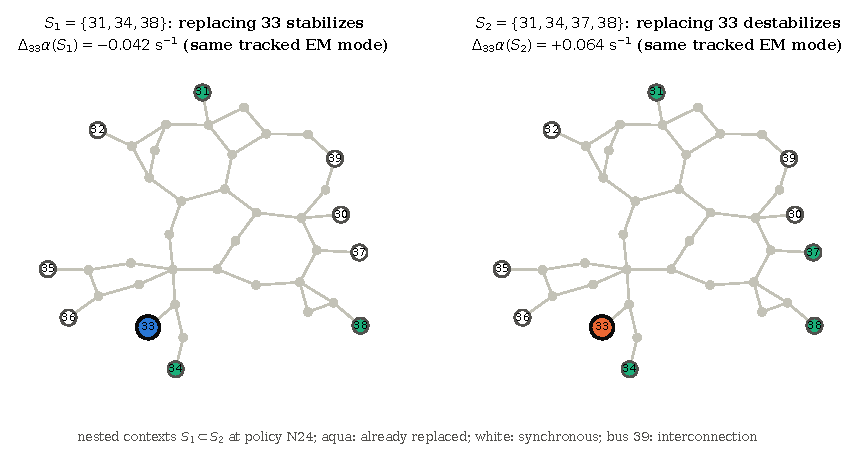
\includegraphics[width=\columnwidth]{CDWH_F1_concept.pdf}
\caption{The same replacement (unit 33) in two nested stable portfolios at
new-holdout policy N24 moves the same tracked EM mode in opposite directions
(orange: destabilizing; blue: stabilizing). Aqua: replaced units; white:
synchronous.}\label{fig:concept}
\end{figure}

The effects are small. Over the \revCpairs{} level-C pairs of base-stable new
policies (\revCdistinct{} distinct unit--policy combinations), reversal magnitudes
$\min(|\Delta_if(S_1)|,|\Delta_if(S_2)|)$ have quartiles
\newCmagQone--\newCmagQthree~s$^{-1}$, or \revZetaQone--\revZetaQthree\,\% of damping
ratio, and the largest is \revCmax~s$^{-1}$. Coverage falls with the threshold
(Fig.~\ref{fig:curv}, right): at 0.02~s$^{-1}$ level C holds in \tauCtwo/19 and
level D in \tauDtwo/19 policies, at 0.03~s$^{-1}$ in \tauCthree/19 and \tauDthree/19,
and at 0.05~s$^{-1}$ in none. Destabilizing$\to$stabilizing reversals dominate: at
level D, s$\to$d occurs in \dirDsd{} and d$\to$s in \dirDds{} policies, and both
directions on one tracked mode in \dirDboth. Converter-parameter draws alone (EC)
remove every EM same-mode reversal from the four-unit lattice at P4 (below).

\begin{figure*}[!t]
\centering
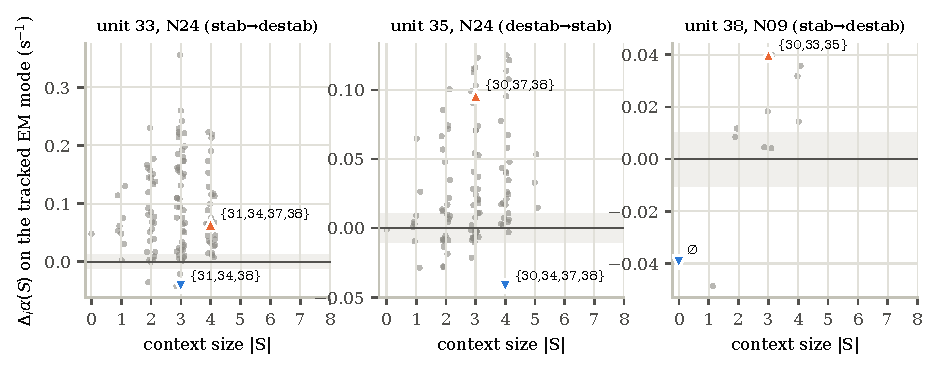
\includegraphics[width=\textwidth]{CDWH_F3_same_mode_examples.pdf}
\caption{Strongest level-D nested reversals on base-stable new-holdout policies
(distinct units). Gray: the unit's level-C contexts; triangles: the nested pair;
band: $\pm\tau_{\rm mat}$.}\label{fig:examples}
\end{figure*}

By Proposition~\ref{prop:abc}, s$\to$d reversals exclude submodularity and d$\to$s
reversals supermodularity; both directions occur at level A in 17 and at level C in
\dirCboth{} of 19 policies. The same conclusion follows directly from one-step
squares whose four portfolios are stable with EM critical modes: second
differences of both signs beyond $10^{-3}$~s$^{-1}$ occur in \emSqNew{} new and
\emSqOld{} old base-stable policies (Fig.~\ref{fig:curv}, left). Fig.~\ref{fig:heat}
maps how often each replacement destabilizes; no unit is uniformly stabilizing or
destabilizing.

\begin{figure*}[!t]
\centering
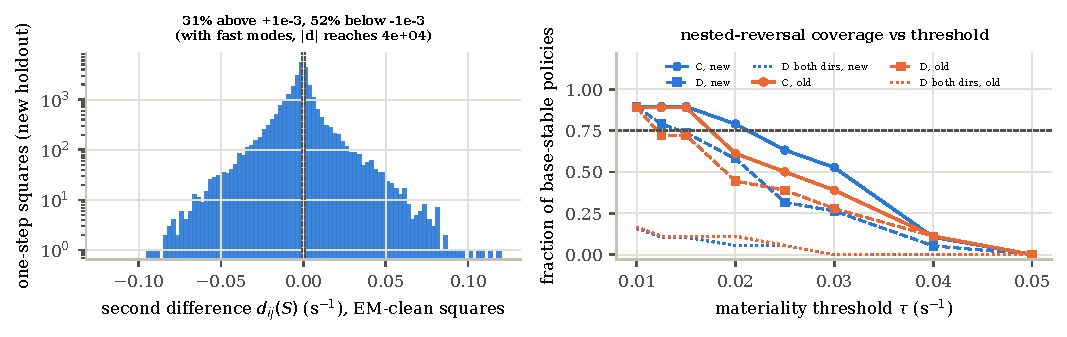
\includegraphics[width=\textwidth]{CDWH_F5_curvature.pdf}
\caption{Left: second differences over one-step squares whose four portfolios are
stable with EM critical modes (new holdout). Right: nested-reversal coverage
against the materiality threshold (level C, level D, and level D in both
directions).}\label{fig:curv}
\end{figure*}

\begin{figure}[!t]
\centering
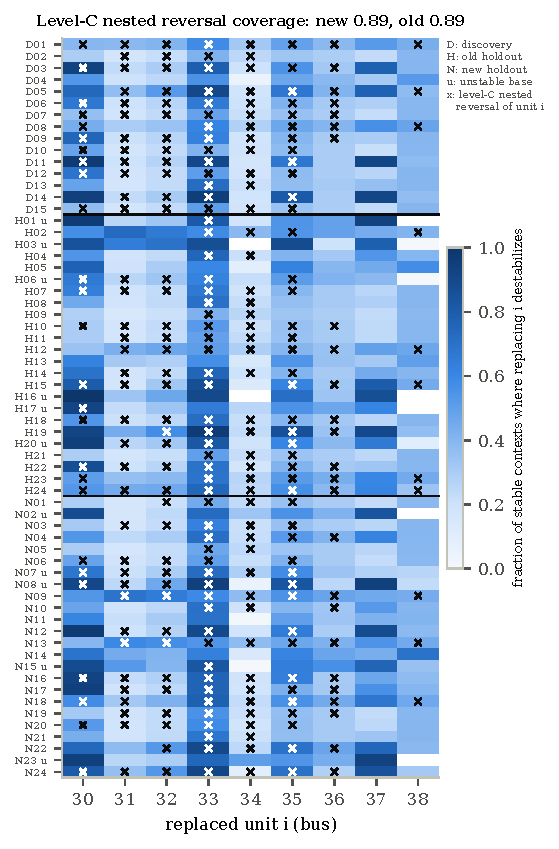
\includegraphics[width=0.80\columnwidth]{CDWH_F2_contextual_reversal.pdf}
\caption{Fraction of stable contexts in which replacing unit $i$ destabilizes,
by policy (D: discovery; H: old holdout; N: new holdout; u: unstable base).
Crosses: level-C nested reversal of unit $i$ (white on dark cells for
contrast).}\label{fig:heat}
\end{figure}

\subsection{Fixed rankings and their anatomy}
The fixed ranking of the nine units that maximizes pairwise agreement with a
policy's own resolved preferences is found exactly by dynamic programming.
Table~\ref{tab:ranking} and Fig.~\ref{fig:ranking} report it. Over all transitions
it orders \pstarFULLNew{} of resolved pairs on the new holdout and its next choice
is at least $\tau_{\rm mat}$ worse than the context-aware choice in \regretFULLNew{}
of stable contexts (\tOneK/\tOneN{} policies have $p^\star<0.90$); the
regret-optimal fixed order, found by a dynamic program over placed prefixes,
reaches \minRegFull. The old-to-new shift is \shiftPstar{} in $p^\star$. A ranking
fitted at one policy errs in \transOffReg{} of decisions at another, against
\transDiagReg{} in sample: the failure is present in sample and transfer adds
little (median Kendall between the policies' optimal orders \orderKendall).

\begin{table}[!t]
\centering
\caption{Oracle-optimal fixed node ranking (medians over base-stable policies). A3 bar: $p^\star\le0.90$ and regret rate $\ge0.10$.}\label{tab:ranking}
\footnotesize
\begin{tabular}{@{}lcccc@{}}
\toprule
& \multicolumn{2}{c}{old holdout} & \multicolumn{2}{c}{new holdout}\\
stratum & $p^\star$ & regret & $p^\star$ & regret \\
\midrule
all transitions & 0.75 & 0.37 & 0.75 & 0.38 \\
EM $\to$ EM transitions & 0.97 & 0.03 & 0.97 & 0.03 \\
EM same-mode (level C) & 0.98 & 0.02 & 0.98 & 0.02 \\
\bottomrule
\end{tabular}
\end{table}


The errors have one source. In \regretNfast{} of the \regretNbad{} materially
wrong decisions (\regretFastShare) the ranked unit pushes the rightmost eigenvalue
out of the EM band; in \noStable{} of the contexts no candidate replacement keeps
the portfolio stable. These out-of-band critical eigenvalues are real in
\fastRealShare{} of cases, with rates of \fastQlo--\fastQhi~s$^{-1}$ (5th--95th
percentile), and appear when five to seven of the nine units are converted.
Their participation concentrates on the converters' PLL angle (\partTheta) and
q-axis current (\partIq). Replacing the added unit fractionally, $\aperp$ jumps
within one 0.025 step of the replaced fraction from about zero to
\sweepJumpLo--\sweepJumpHi~s$^{-1}$, exactly where the smallest singular value of
$g_z$ reaches \sweepSigLo--\sweepSigHi{} (six sweeps, supplement): the signature of a
singularity-induced bifurcation of the DAE~\cite{venkatasubramanian1995sib}. These
events mark a loss of the index-one property of the phasor model at high
converter share; their physical course would require network dynamics or an EMT
model, which were not used. Restricted to transitions that stay in the EM band, the
oracle ranking orders \pstarEMNew{} of pairs and errs in \regretEMNew{}, failing the
preregistered insufficiency bar; screening the ranking for stability (first ranked
unit whose next portfolio is stable) lowers its regret from \regPlainFeas{} to
\regScreened{} on contexts with a stable option. A portfolio-conditioned static
screen, choosing the unit that maximizes the generalized SCR of $S\cup\{i\}$, errs
in \gscrSeqFull{} of decisions.

\begin{figure*}[!t]
\centering
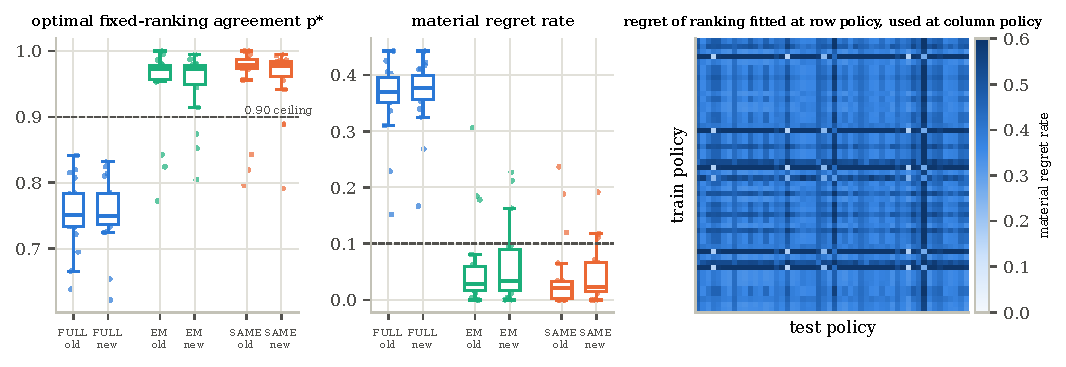
\includegraphics[width=\textwidth]{CDWH_F4_fixed_ranking.pdf}
\caption{Agreement-optimal fixed ranking: agreement $p^\star$ and material regret
rate by stratum (old and new holdout), and regret of rankings transferred
between base-stable policies (rows: policy of fit; columns: policy of use,
ordered discovery, old, new).}\label{fig:ranking}
\end{figure*}

\begin{table}[!t]
\centering
\caption{Preregistered evidence layers for ``a context-independent node ranking does not suffice'' (new holdout). Strong claim: $\ge5$ of 8 including L2 and L5.}\label{tab:layers}
\scriptsize
\setlength{\tabcolsep}{2pt}
\begin{tabular}{@{}cL{0.44\columnwidth}L{0.36\columnwidth}c@{}}
\toprule
& layer & value & pos. \\
\midrule
L1 & arbitrary-context reversal & 1.00 & yes \\
L2 & nested-context reversal (level A) & 1.00 & yes \\
L3 & same-mode nested reversal (level B) & 0.95 & yes \\
L4 & EM same-mode nested reversal (level C) & 0.89 & yes \\
L5 & optimal fixed ranking failure (FULL) & p*=0.749; regret=0.376 & yes \\
L6 & ranking transfer failure & offdiag regret=0.402; diag=0.376 & yes \\
L7 & envelope robustness (fresh draws) & EC: 1.0, EM-f: 0.9, EM-u: 0.8, EMC: 1.0 & yes \\
L8 & dynamic-converter holdout (ALT-WECC reversal) & 0.0 (MODEL-SPECIFIC) & no \\
\bottomrule
\end{tabular}
\end{table}


The preregistered evidence layers (Table~\ref{tab:layers}) meet the frozen rule
for the claim that a context-independent node ranking does not suffice (7 of 8
positive), but the layers are nested and the ranking layers do not survive the EM
restriction; we read the result as: in this model a fixed list fails because it
cannot anticipate which replacement crosses the singularity, and within stable EM
dynamics it is a reasonable approximation.

\subsection{Portfolio-conditioned reinforcement ranking}
Table~\ref{tab:goldb} and Fig.~\ref{fig:goldb} report branch ranking for the core
portfolio $V_4$. On the \nElig{} preregistration-eligible conditions (equilibrium
residual $\le10^{-8}$, a threshold below the solver's residual of order
$10^{-7}$ in most conditions; six of the eight are draws at P4), the median Spearman
correlation with the finite $\times1.5$ outcome is \gbpreregmedianrhoDtotal{} for
$\Dtot$, \gbpreregmedianrhoDfrozen{} for $\Dfro$ and \gbpreregmedianrhoSone{} for
$|P_e|$, with paired advantage \gbpreregmediandiff{} (interval
\gbPreregCiLo--\gbPreregCiHi) and top-5 precision \gbpreregmediantopfiveDtotal{};
the preregistered gate passes, while the secondary test T2 does not reach
$p<0.05$ with six clusters. Over all 64 solved conditions (residual
$\le$\rZeroMax) the medians are \gbprimarymedianrhoDtotal, \gbprimarymedianrhoDfrozen{}
and \gbprimarymedianrhoSone.

\begin{table}[!t]
\centering
\caption{Branch-reinforcement ranking on the new holdout (target H4, truth: finite re-equilibrated $\times1.5$). Medians over conditions; ``elig.'': the 8 preregistration-eligible conditions ($R_0\le10^{-8}$); other columns: all 64 solved conditions.}\label{tab:goldb}
\scriptsize
\setlength{\tabcolsep}{2.2pt}
\begin{tabular}{@{}lcccccc@{}}
\toprule
predictor & $\rho$ elig. & $\rho$ & $\tau$ & concord. & top-5 & NDCG@5 \\
\midrule
$|P_e|$ (S1, selected) & 0.49 & 0.50 & 0.39 & 0.71 & 0.20 & 0.61 \\
$|S_e|$ & 0.47 & 0.48 & 0.37 & 0.69 & 0.20 & 0.61 \\
$|z_e|$ & 0.25 & 0.24 & 0.20 & 0.61 & 0.20 & 0.27 \\
electrical distance & 0.21 & 0.19 & 0.15 & 0.58 & 0.40 & 0.38 \\
effective resistance & 0.30 & 0.30 & 0.22 & 0.61 & 0.60 & 0.58 \\
Fiedler edge score & -0.05 & -0.05 & -0.03 & 0.48 & 0.20 & 0.36 \\
edge betweenness & -0.28 & -0.27 & -0.18 & 0.40 & 0.00 & 0.17 \\
endpoint $dV/dQ$ & -0.17 & -0.16 & -0.10 & 0.45 & 0.00 & 0.16 \\
$\Delta$gSCR(H4) & 0.16 & 0.17 & 0.12 & 0.57 & 0.20 & 0.30 \\
\midrule
base-portfolio eig.\ sens. & -0.05 & 0.03 & 0.01 & 0.50 & 0.60 & 0.91 \\
frozen (portfolio) & 0.91 & 0.90 & 0.77 & 0.90 & 0.60 & 0.97 \\
\textbf{total (portfolio)} & \textbf{0.98} & \textbf{0.99} & \textbf{0.93} & \textbf{0.98} & \textbf{1.00} & \textbf{0.99} \\
port form (policies only) & 0.99 & 1.00 & 0.96 & 1.00 & 1.00 & 1.00 \\
\bottomrule
\end{tabular}
\end{table}


The informative comparisons are with $\Dfro$ and with a fixed list. Across the 24
new policies, $\Dtot$ has median Spearman \gbnewpoliciesmedianrhoDtotal, $\Dfro$
\gbnewpoliciesmedianrhoDfrozen{} and the learned fixed list \locoNew; across the
40 draws at P4 the list reaches \locoDraws{} against \gbfreshdrawsmedianrhoDtotal.
$\Dtot$ exceeds the list in every condition, but the median paired margin is \locoMarginDraws{} on
the draws and \locoMarginNew{} on the new policies, not the 0.5 gap to static indices, which do
not respond to conditions at all. The
branch ranking thus changes mostly across controller policies. $\Dtot$ also ranks
large actions: at \dtotTopoNpol{} new-holdout policies, Spearman with the finite effect of
doubling a branch is \dtotDbl{} and of removing it \dtotOut{} (top-5 \dtotOutTop).
The first-order prediction overstates the largest reinforcements, whose effect
saturates at $\gamma_e=1.5$ (Fig.~\ref{fig:goldb}, right). The port form in
Table~\ref{tab:goldb} re-derives $\Dtot$ from re-solved Jacobians and is a
verification, not an independent method.

\begin{figure*}[!t]
\centering
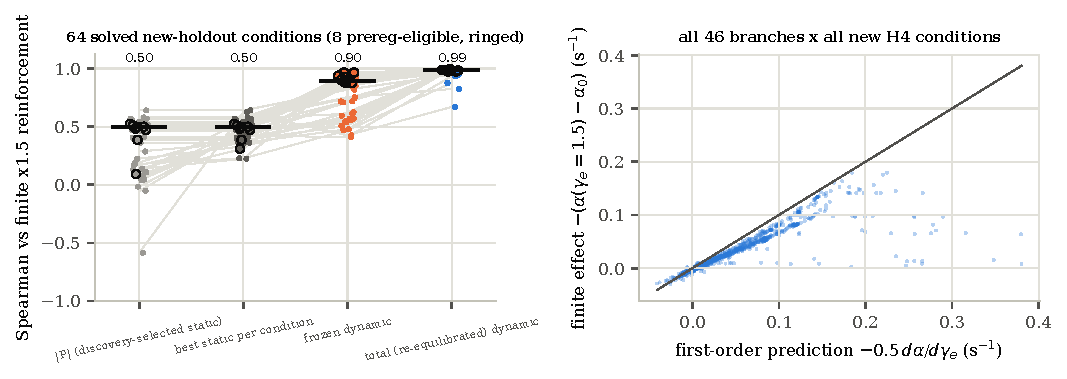
\includegraphics[width=\textwidth]{CDWH_F6_goldb.pdf}
\caption{Left: Spearman correlation with the finite reinforcement outcome per
new-holdout condition (lines join the same condition; ringed: the
preregistration-eligible subset). Right: first-order prediction vs finite
effect, all branches and conditions.}\label{fig:goldb}
\end{figure*}

\subsection{When re-equilibration matters}
Splitting \eqref{eq:tot} into frozen and re-equilibration parts
(Fig.~\ref{fig:why}): for $g_i$, PLL scales and AVR gains the two derivatives agree
to \nodeRone{} relative, as the remark predicts. For loads the re-equilibration
term exceeds the frozen term in \nodeLoadDom{} of cases. For branches it exceeds
the frozen term for about half of the branches and changes the ranking materially
(sign disagreement $\ge10$\,\% or Kendall $\le0.6$) in \heightMaterial{} of the $V_4$
conditions; every condition has a branch whose frozen and total signs differ.

\begin{figure*}[!t]
\centering
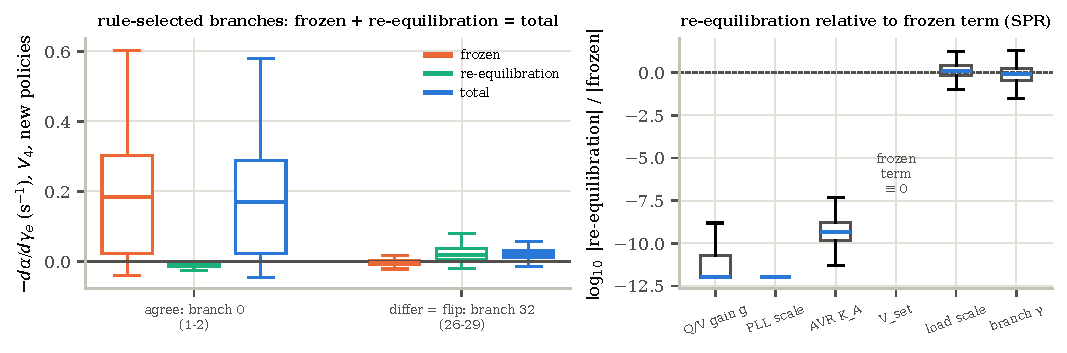
\includegraphics[width=\textwidth]{CDWH_F7_why_total.pdf}
\caption{Left: frozen, re-equilibration and total branch sensitivities for the
branches selected by the preregistered rule. Right: ratio of the
re-equilibration term to the frozen term by coordinate class (the frozen term of
voltage setpoints is identically zero).}\label{fig:why}
\end{figure*}

\subsection{Robustness to parameter draws}
Under the fresh envelope draws at P4 the coverage of a stable-context reversal on
the four-unit lattice is \lSevenEC{} (EC), \lSevenEMf{} (EM-f), \lSevenEMu{} (EM-u)
and \lSevenEMC{} (EMC); for EM same-mode reversals it is \lSevenEMEC, \lSevenEMEMf,
\lSevenEMEMu{} and \lSevenEMEMC. The EM reversals are therefore sensitive to the
converter parameters. Branch ranking on the draws gives median $\rho$
\gbfreshdrawsmedianrhoDtotal{} for $\Dtot$ and \gbfreshdrawsmedianrhoSone{} for $|P_e|$.

\subsection{Cross-model holdout}\label{sec:cross}
Table~\ref{tab:cross} summarizes ALT-WECC on the seven preregistered policies
with a stable ALT base. Its converted portfolios are less stable than with the
custom GFL; $V_4$ is unstable at all policies. The preregistered test on the
global $\aperp$ finds no stable-context reversal, but it is uninformative: in
most stable ALT portfolios $\aperp$ is set at $-0.100$~s$^{-1}$ by the anti-windup
tracking state of the plant-level active-power integrator, a state decoupled
from the rest of the model that our structural rule kept. On the tracked EM mode,
stabilizing replacements occur at \altEmStab{} of \altEmN{} policies and a nested reversal at \altEmRev{} of
\altEmN{} (\altEmPol), the same policy at which the custom GFL has a level-C reversal on this
lattice.
Switching on the library's voltage control (all gains unchanged, post hoc) gives
no stabilizing replacement and no reversal, so the data do not support the
reading that converter voltage control is what enables reversals. The 12-branch
finite ranking is model-specific (median Kendall \altCMedianKendall), as a previous
cross-tool check had indicated, while within ALT-WECC a finite-difference total
sensitivity ranks the model's own outcomes at \altCMedianRhoAltfd{} against
\altCMedianRhoS{} for $|P_e|$, a margin at the preregistered bar. Top-1 agreement
of the equal-budget corridors (Section~\ref{sec:corr}) is partial (\altDFracTopAgree) and the
topology directions agree (\altEPooledSignAgree{} on \altENPairs{} pairs).

\begin{table}[!t]
\centering
\caption{Cross-model holdout: frozen TX3 WECC library GFL chain (ALT-WECC, ANDES) vs the custom GFL, 8 preregistered policies.}\label{tab:cross}
\footnotesize
\setlength{\tabcolsep}{2.5pt}
\begin{tabular}{@{}cL{0.37\columnwidth}L{0.28\columnwidth}L{0.20\columnwidth}@{}}
\toprule
& test & value & verdict \\
\midrule
A & stable-context reversal, core lattice & 0.00 of 7 (custom 0.71) & model-specific \\
B & same-mode reversal & 0.00 & model-specific \\
C & 12-line finite ranking, Kendall custom vs ALT & median 0.02 & model-specific \\
C2 & ALT total vs ALT finite, minus $|P|$ & 0.99 vs 0.79 & transfers \\
D & corridor top-1 agreement & 0.75 & transfers \\
E & topology sign agreement & 0.94 (35 pairs) & transfers \\
\bottomrule
\end{tabular}
\end{table}


\subsection{Topology and electromechanical modes}
Topology effects were re-evaluated by tracking the pre-action EM-band rightmost
mode of each portfolio through every admissible action (Fig.~\ref{fig:topo});
events in which the full $\aperp$ is set by a non-EM mode and differs from the
tracked change (\topoFastHfour{} of 1296 $V_4$ policy--action cases) are excluded. At
P4, doubling any one of lines 1--2, 1--39, 8--9 or the 23--36 transformer makes
$V_4$ stable; across the 16 policies, \topoNcreate{} (policy, action) pairs create an
EM-failing hyperedge of at most three units, all by outages and all but three at
discovery or old-holdout policies (\creDisc{} and \creOld). No static topology score
meets the prediction rule ($|\rho|\ge0.6$ in $\ge75$\,\% of policies); their median
correlations of about $\pm0.5$ come from separating outages from doublings, and
within doublings they are near zero (Fiedler value \withinDblFiedler). This is
expected N$-$1 small-signal behavior and we report it as a supporting observation.

\begin{figure*}[!t]
\centering
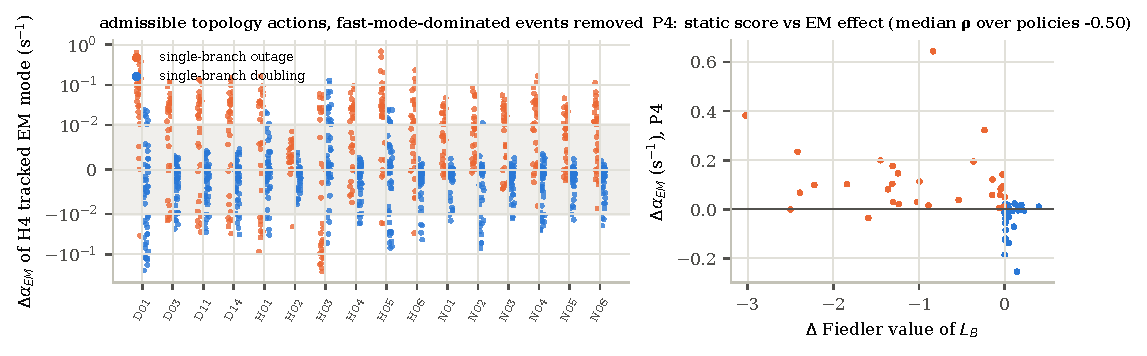
\includegraphics[width=\textwidth]{CDWH_F8_topology_em.pdf}
\caption{Left: tracked EM-mode change of $V_4$ for every admissible action, by
policy (fast-mode-dominated events removed; band: $\pm\tau_{\rm mat}$). Right: at
P4, EM effect against the change of the Fiedler value.}\label{fig:topo}
\end{figure*}

% corridor subsection: generated after H10


\subsection{Modal mixing is not confirmed}
A first campaign reported that controller-weighted modal mixing of the network
port operator correlates with the number of reversing units ($\rho=\mixOldOrigRho$ on
the old holdout), evaluated at each policy's own critical frequency. At a fixed
reference frequency the old-holdout correlation falls to \mixOldFixedRho; on the new
holdout the preregistered test gives $\rho=\mixNewRho$ ($p=\mixNewP$, Holm
\tThreePholm), which misses the bar $p\le0.01$ (with 19 policies the test has
little power at this effect size). In an exact two-factor decomposition of the
mixing change, the controller term carries \mixVarCtrl{} and the frequency term
\mixVarFreq{} of the variance, with a covariance term of \mixCov.

% =========================================================================
\section{Discussion}\label{sec:discussion}

\emph{What a planner needs.} On this benchmark, choosing the next unit in context
is cheap: nine eigenanalyses per step. The practical content of C2 is therefore
diagnostic: a fixed weak-bus list is unreliable because it cannot anticipate which
replacement crosses the high-share singularity, and a stability check per
candidate---which is exactly an in-context evaluation---removes most of that
failure, while a portfolio-conditioned gSCR screen does not. For reinforcement,
the result is that the re-equilibrated sensitivity of the planned portfolio ranks
reinforcements, doublings and outages reliably, that the frozen derivative
degrades across controller policies, and that a list learned from other
conditions is good but not adequate across policies. We do not claim a
computational saving: our implementation evaluates the total derivative with
finite-difference Jacobians at \timeDer~s per branch, against \timeFin~s for a
finite re-solve and eigenanalysis; a saving would require analytic second
derivatives and large systems, which we did not test.

\emph{Relation to strength metrics and placement.} Static indices are
computed from the base network and do not respond to the policy or the draw; they
carry some information (effective resistance places three of the five strongest
branches in its top five) but do not order reinforcements within a portfolio.
Placement methods built on grid-strength or Kron-reduced-Laplacian surrogates
treat converters as homogeneous and, for grid-forming conversions, can show that
each conversion helps~\cite{yang2021gfm,xin2025howmany,huang2022gridstructure};
the reversals here arise with heterogeneous machines and a converter with its own
Q/V control, and they were not reproduced by the library converter. Offline
priority lists of switching actions~\cite{khaji2017switching} are fixed rankings
of the kind examined in Section~\ref{sec:results}-B.

\emph{Literature scope.} The gap statements rest on a focused search of
2020--2026 journal and conference records, extended to the earlier displacement
literature, with arXiv only where no peer-reviewed version exists and without
full-text database access; they state the absence of such results within that
search.

\emph{Limitations.} All results are phasor-domain small-signal results on one
network with one custom GFL and one parameter box; the holdout tests robustness to
controller coordinates, not generality. The machines have $D=0$ and no governors,
loads are constant power, and dispatch is matched; realistic damping, governors,
voltage-dependent loads or unmatched reactive dispatch could remove the small
stabilizing side of many reversals, and they were not tested. The fast events
behind the fixed-ranking failure are singularity crossings of an idealized phasor
converter without current limits. The EM reversals are sensitive to converter
parameters and are not reproduced by the library converter. The primary GOLD-B set
has eight conditions because the preregistered residual threshold was stricter than
the solver tolerance. The deviation log records execution fixes, post-hoc
analyses, a defect in the cross-model tests found by internal review, and hand-written
clock times that were later corrected against the commit history.

% =========================================================================
\section{Conclusion}
On the IEEE 39-bus benchmark, the small-signal effect of replacing an SG by a GFL
depends on the portfolio in which it occurs: nested reversals on the same
electromechanical mode recur on a preregistered holdout, at magnitudes of about
one hundredth of s$^{-1}$. A fixed ranking of units fails mainly because it cannot
anticipate aperiodic singularity crossings at high converter share; with a
stability screen it is nearly adequate. The re-equilibrated eigenvalue
sensitivity of the planned portfolio ranks branch reinforcements, doublings and
outages better than frozen derivatives, fixed lists and static indices, and this
method, unlike the specific ranking, carries over to a library converter model.
Reinforcement rankings should be recomputed for the portfolio and controller
settings in which they are applied.

\section*{Data and code availability}
Preregistration, deviation log, code, result tables and figure sources are in the
project repository, branch \texttt{research/}\allowbreak
\texttt{contextual-dynamic-weakness-hardening}; software: Python 3.13, NumPy 2.5,
SciPy 1.18, ANDES 2.0.

\bibliographystyle{IEEEtran}
\bibliography{references}

\end{document}
